\section{Multivariate analysis}

The event selection described in~\Cref{sec:event_selection} only
serves as a preselection with the intention that selected events
follow the expected topology of the signal and that basic kinematic
requirements, ensuring trigger efficiencies are in saturation, are
fulfilled.\todo{Say something about signal to background ratio}

The non-resonant and resonant production of SM Higgs boson pairs have
distinct kinematic properties that can be used to reject backgrounds
in the signal region. An example that is independent of the production
mode of SM Higgs boson pairs is the invariant mass of the \bbbar pair
and the \hadhad which can be reconstructed. A number of reconstructed
quantities can be defined that offer discrimination power to
distinguish between the various signals and backgrounds.

Multivariate methods are employed to exploit the discrimination power
of multiple reconstructed quantities and their correlations to
classify events regarding their signal- and
background-likeness. Depending on the \HH production mode and analysis
category different methods are used.

The search of non-resonant \HH production in the SM uses Boosted
Decision Trees and Neural Networks to distinguish between signal and
background in the \hadhad and \lephad channel, respectively. When
searching for resonant \HH production in BSM scenarios, multiple mass
hypotheses for the scalar resonance decaying into SM Higgs boson pairs
are considered. The signal event kinematics are therefore dependent on
the mass of the resonance, \mX, and as a result the classification
task continuously varies as a function of \mX. This is in contrast to
the former case where the kinematic properties of signal events are
fixed. Classification tasks that vary as a function of a parameter,
for example the resonance mass, can be performed by \emph{Parametric
  Neural Networks} (PNN), first introduced to HEP
in~\cite{Baldi:2016fzo}. PNN provide a single classifier that is able
to handle multiple classification tasks, while being able to smoothly
interpolate the parameter to values not seen during training.

The scores provided by these multivariate classification methods,
hereafter called MVA scores, are later used as a discriminant in the
maximum likelihood fit to extract the signal of interest and set upper
limits on signal strengths and cross-sections. No further selections
are applied to events entering the signal extraction procedure such
that the preselection regions are also the signal regions in the
respective channels.

In~\Cref{sec:mva_discriminating variables} the choice of
discriminating variables to classify signal and background processes
will be motivated. Afterwards, the training and optimisation of the
classifiers used to extract non-resonant signal is described
in~\Cref{sec:mva_smbdt}. Finally, \Cref{sec:mva_pnn} will explain the
interpolation properties of PNN as well as the training and
optimisation procedures used. \todo{Variable importance?}


\subsection{Cross validation method}
\label{sec:mva_crossvalidation}

Many machine learning algorithms, due to their ability to approximate
large classes of functions, are susceptible to fitting statistical
fluctuations in the data that are used to train a model. As a result,
predictions of performance characteristics of the model based on the
training data might not generalise to previously unseen data. In
extreme cases, frequently called overfitting, the performance of the
model evaluated on an independent dataset starts to degrade when
further increasing the capacity of the model~\cite{hastie09}.

When using multivariate methods in measurements or searches for new
physics, it has to be ensured that the methods are evaluated on a
dataset that was not used for training or model selection (the process
of choosing the model to fit), thus providing an estimator of the
generalised performance. In this analysis, events are categorised
according to their event number into even- and odd-numbered events,
yielding an even- and odd-fold, respectively. The training and model
selection can proceed by using one of the two folds withholding the
remaining fold for later evaluation. This procedure is applied twice
by using each fold for training once.

After model selection and training, the models are evaluated by
applying the model trained on the even-fold on odd-numbered events and
the model trained on the odd-fold on even-numbered events. This
approach, which is called two-fold \emph{cross
  validation}~\cite{hastie09,bishop06}, provides an unbiased
evaluation of the MVA scores using the entirety of the available
dataset. The same evaluation method is applied to signal region data
recorded by the ATLAS detector, which is not part of the training
procedure.

Similar to the biased predictions obtained when evaluating
multivariate methods on datasets used for training, the process of
model selection needs to be performed on a dataset that is independent
of the one used for final evaluation of the
method~\cite{cawley10}. Model selection is the process of choosing a
particular configuration of the algorithm, for example input variables
and other hyperparameters, based on a metric indicating the
performance of the model.

The model selection is performed by using five-fold cross validation
(CV), which is a generalisation of the two-fold approach described
previously to a larger number of subdivisions, separately on the even-
and the odd-numbered events. This approach effectively nests five-fold
CV inside of two-fold CV and is therefore called \emph{nested cross
  validation}~\cite{cawley10,stone74}.

\Cref{fig:cross_validation} shows a schematic description of one
iteration of the nested cross validation approach. The inner,
five-fold CV randomly splits events into five disjoint subsets
(folds). For every choice of fold used to evaluate the model, the
model is trained on the remaining four folds, subsequently evaluating
the trained model on the evaluation-fold. A decision between two
competing models can be made by comparing the average and standard
deviation of the evaluation metric over the five iterations of the
inner CV. Only after the best-performing model is selected, usually
after re-fitting the model on all five folds, it is evaluated on the
hold-out dataset.

\begin{figure}[htbp]
  \centering

  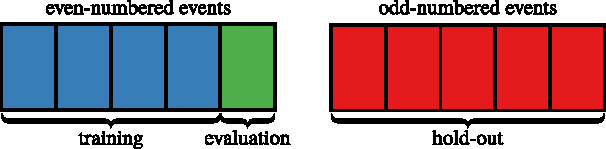
\includegraphics[scale=1]{mva/kfold}

  \caption{Five-fold cross validation approach for model selection on
    even-numbered events. The separation of events into disjoint
    subsets (folds) is indicated by rectangles. The purpose of the
    subset is denoted below. A single step out of a total of five, the
    number of possible assignments of the evaluation fold, is
    shown. The hold-out dataset is not used for model selection.}
  \label{fig:cross_validation}
\end{figure}


\subsection{Discriminating variables}
\label{sec:mva_discriminating variables}

The set of variables provided to multivariate classification methods
is crucial to its performance in distinguishing between classes. The
initial choice of variables considered in this search was based on a
previous publication in the same analysis channel by the ATLAS
collaboration using a partial dataset of \SI{36.1}{\ifb} recorded
during Run~2~\cite{HIGG-2016-16-witherratum}.

The pair production of SM Higgs bosons has kinematic features that
allow to distinguish it from the main backgrounds in the $\bbtautau$
search channel. Candidates for the products of
$\PHiggs \ra \Pbottom\APbottom$ and $\PHiggs \ra \Ptauon\APtauon$
decays are reconstructed (cf.~\Cref{sec:}) and can be used to estimate
properties of the SM Higgs bosons in signal processes. Among the most
important variables distinguishing between signal and background
processes are \PHiggs- and \HH-system invariant masses.

The Missing Mass Calculator (MMC)~\cite{Elagin:2010aw} is used to
reconstruct the four-momentum of the Higgs candidate decaying into
pairs of \tauleptons, providing an estimate of the $\tau\tau$-system
mass, \mMMC. For the signal processes in the \hadhad
channel\footnote{The presence of an additional neutrino in the \lephad
  channel makes mass reconstruction of the $\tau\tau$-system more
  difficult degrading the resolution.}, \mMMC provides an estimate of
the Higgs boson mass with a resolution\todo{Is this the right word?}
of \SIrange{15}{18}{\GeV} depending on the momentum of the Higgs
boson. Similarly, the mass of the $\PHiggs \ra \Pbottom\APbottom$
candidate, consisting of two \btagged jets, is reconstructed from the
four-momenta of the jets after $b$-jet momentum correction
(cf.~\Cref{sec:}). In this case, the Higgs boson mass can be
reconstructed with a resolution of \SIrange{13}{18}{\GeV}.\todo{Does
  it make sense to call this a resolution?}

The performance of the \PHiggs mass reconstruction is summarised
in~\Cref{fig:mass_reconstruction_H} for the resonant production of
Higgs boson pairs as a function of the resonance mass. In conjunction,
the narrow mass peaks in \mMMC and \mBB expected for the signal
processes provide large rejection power against most
backgrounds. Therefore, \mMMC and \mBB are used as inputs to the MVAs
in all analysis categories.

\todo{Move to event selection section?}

\begin{figure}[htbp]
  \centering

  \begin{subfigure}[t]{.5\textwidth}
    \centering
    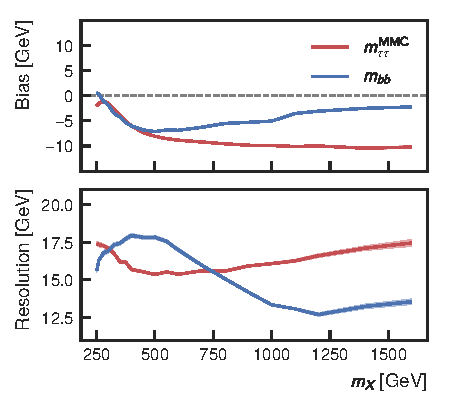
\includegraphics{mva/mass_resolution}
    \caption{\PHiggs-system mass reconstruction}
    \label{fig:mass_reconstruction_H}
  \end{subfigure}\hfill%
  \begin{subfigure}[t]{.5\textwidth}
    \centering
    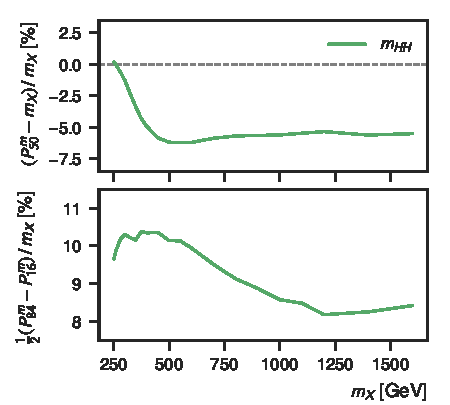
\includegraphics{mva/mhh_resolution}
    \caption{\HH-system mass reconstruction}
    \label{fig:mass_reconstruction_HH}
  \end{subfigure}

  \caption{Performance of methods used to reconstruct the
    \PHiggs-system mass (a) and the \HH-system mass (b) in the \hadhad
    SR estimated using simulation of $\PX \ra \HH \ra \bbtautau$
    processes. The top panels show the median mass prediction,
    $P_{50}^{m}$, of the respective method. The bottom panels show
    half the difference between the 84th and 16th percentile as an
    estimate of the resolution. For the \HH-system reconstruction,
    these quantities are shown relative to the mass of the resonance.}
  \todo[inline]{Add error. Should say sth.\ about the bias and
    behaviour.}
  \label{fig:mass_reconstruction}
\end{figure}

The invariant mass of the decay products of both Higgs bosons, \mHH,
provides another discriminant used in all analysis categories. It is
determined from the sum of four-momenta of $\Ptauon\APtauon$-system,
reconstructed using the MMC, and $\bbbar$-system, calculated as the
sum of $b$-jet candidate four-momenta after $b$-jet momentum
correction. With a peak width of \SIrange{8}{10}{\percent} relative to
the mass of the resonance and the prevalence of most backgrounds at
low values of \mHH, it provides an important discriminant for the
search in the resonant production mode.

With the exception of resonant production with low \mX, Higgs bosons
originating from the signal processes are typically produced with
large momentum in the \HH rest frame. As a result, the angular
separation of the (visible) \PHiggs decay products is small. The
Lorentz-invariant angular distances \dRtautau and \dRbb between the
visible decay products of the \taulepton and $b$-jet candidate pair,
respecively, provide discrimination power against multi-jet and top
pair production. % , except for \dRbb in \lephad LTT,

In a given analysis category, the same input variables are used in
MVAs used to extract the resonant and non-resonant \HH signal. The
choice of variables differs between categories and is summarised
in~\Cref{tab:mva_inputvar}. A brief description of variables used in
the \lephad channel is given in the following. When referring to
leptons, $\ell$, only electrons or muons are implied.\nopagebreak
\begin{description}

\item[$\Delta \pT(\ell, \tauhadvis)$] The transverse momentum
  difference between lepton and \tauhadvis.

\item[\mTW] Transverse mass of the \PW boson for processes where
  \pTmiss solely originates from the decay $\PW \ra \ell \nu_\ell$ defined as:
  $\mTW = \sqrt{2 |\pT^{\ell}| |\pTmiss| \cos(1 - \Delta\phi)}$.

\item[\pTmiss $\phi$ centrality] A measure of the relative angular
  position of \pTmiss and visible \taulepton decay products
  (electrons, muons, or \tauhadvis) in the transverse plane. The
  measurement is relative to the line bisecting the azimuthal angle
  between the pair of visible \taulepton decay products and can be
  defined as~\cite{HIGG-2013-32, HIGG-2016-16-witherratum}:
  \begin{align*}
    \pTmiss\text{ }\phi\text{ centrality} = \frac{A + B}{\sqrt{A^2 + B^2}} \text{,}
  \end{align*}
  where
  \begin{align*}
    A = \frac{\sin(\phi_{\pTmiss} - \phi_{\tau_1})}{\sin(\phi_{\tau_2} - \phi_{\tau_1})} \qquad B = \frac{\sin(\phi_{\tau_2} - \phi_{\pTmiss})}{\sin(\phi_{\tau_2} - \phi_{\tau_1})} \text{,}
  \end{align*}
  with $\phi_{\pTmiss}$ and $\phi_{\tau_1}$ / $\phi_{\tau_2}$ denoting
  the azimuthal angle of \pTmiss and visible \taulepton decay
  products, respectively.

  The \pTmiss $\phi$ centrality reaches a maximum of $\sqrt{2}$
  (minimum of $-\sqrt{2}$) when \pTmiss is aligned with the bisecting
  line, pointing into the smaller (larger) angle spanned by the pair
  of visible \taulepton decay products. In configurations where
  \pTmiss is collinear with one of the visible \taulepton decay
  products it takes a value of 1.

\item[$\Delta\phi(\ell\tauhadvis, bb)$] Azimuthal angle between the
  $\ell + \tauhadvis$ system and the system consisting of the two
  \bjet candidates.

\item[$\Delta\phi(\ell, \pTmiss)$] Azimuthal angle between the lepton
  and \pTmiss.

\item[$\Delta\phi(\pTauTau, \pTmiss)$] Azimuthal angle between
  $\tau\tau$-system, reconstructed using the MMC, and \pTmiss.

\item[$s_{\text{T}}$] The effective mass of the event defined as the
  scalar sum of tranverse momenta of all selected jets, \tauhadvis,
  leptons, and \pTmissAbs.
\end{description}

\begin{table}[htbp]
  \centering

  \begin{tabular}{
  l
  >{\centering\arraybackslash}p{2cm}
  >{\centering\arraybackslash}p{2cm}
  >{\centering\arraybackslash}p{2cm}
  }
  \toprule
  & \multicolumn{3}{c}{Analysis Channel} \\ \cmidrule{2-4}
  Variable                              & \hadhad    & \lephad SLT & \lephad LTT \\
  \midrule
  \mMMC                                 & \checkmark & \checkmark & \checkmark \\[0.1em]
  \mBB                                  & \checkmark & \checkmark & \checkmark \\[0.1em]
  \mHH                                  & \checkmark & \checkmark & \checkmark \\[0.1em]
  \dRtautau                             & \checkmark & \checkmark & \checkmark \\[0.1em]
  \dRbb                                 & \checkmark & \checkmark &            \\[0.1em]
  $\Delta \pT(\ell, \tauhadvis)$        &            & \checkmark & \checkmark \\[0.1em]
  Sub-leading $b$-jet \pT               &            & \checkmark &            \\[0.1em]
  \mTW                                  &            & \checkmark &            \\[0.1em]
  \pTmissAbs                            &            & \checkmark &            \\[0.1em]
  \pTmiss $\phi$ centrality             &            & \checkmark &            \\[0.1em]
  $\Delta\phi(\ell\tauhadvis, bb)$      &            & \checkmark &            \\[0.1em]
  $\Delta\phi(\ell, \pTmiss)$           &            &            & \checkmark \\[0.1em]
  $\Delta\phi(\pTauTau, \pTmiss)$       &            &            & \checkmark \\[0.1em]
  $s_{\text{T}}$                         &            &            & \checkmark \\
  \bottomrule
 \end{tabular}


%%% Local Variables:
%%% mode: latex
%%% TeX-master: "../phd_thesis.tex"
%%% End:


  \caption{Discriminating variables used by the multivariate methods
    to extract the non-resonant and resonant \HH signals in the
    \hadhad, \lephad SLT, and \lephad LTT channels.}
  \label{tab:mva_inputvar}
\end{table}

The \pTmiss $\phi$ centrality, used in the \hadhad channel of the
previous publication~\cite{HIGG-2016-16-witherratum}, was not found to
contribute to the classification performance when comparing models
with cross validation (cf.~\Cref{sec:mva_crossvalidation}) in the
\hadhad channel. It is therefore removed as an input to the
multivariate analysis of the \hadhad channel.

The five discriminating variables used in the \hadhad channel are
shown in~\Cref{fig:mva_inputs}. A selection of variables in the
\lephad SLT and LTT channels are documented
in~\cite{ATLAS-CONF-2021-030}.

\begin{figure}[htbp]
  \centering

  \begin{subfigure}[t]{.48\textwidth}
    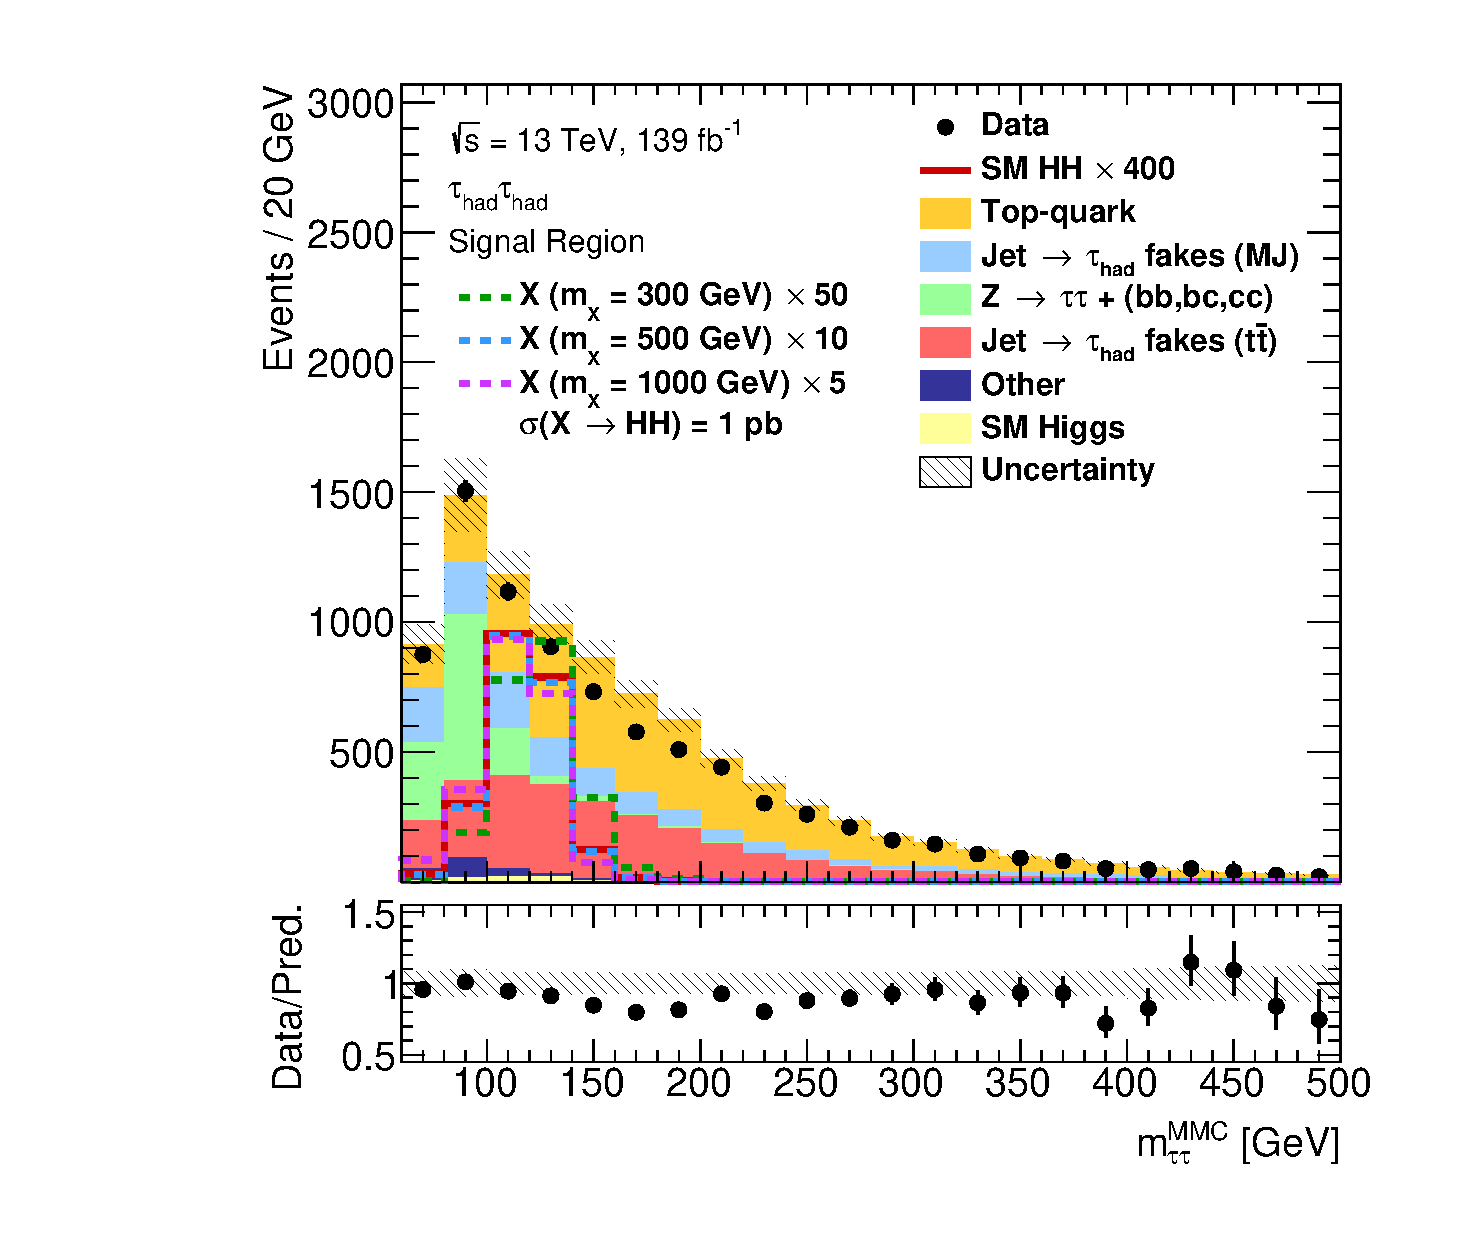
\includegraphics[width=\textwidth]{mva/prefit/Region_BMin0_incJet1_distmMMC_J2_Y2015_DLLOS_T2_SpcTauHH_L0_Prefit}
  \end{subfigure}\hfill %
  \begin{subfigure}[t]{.48\textwidth}
    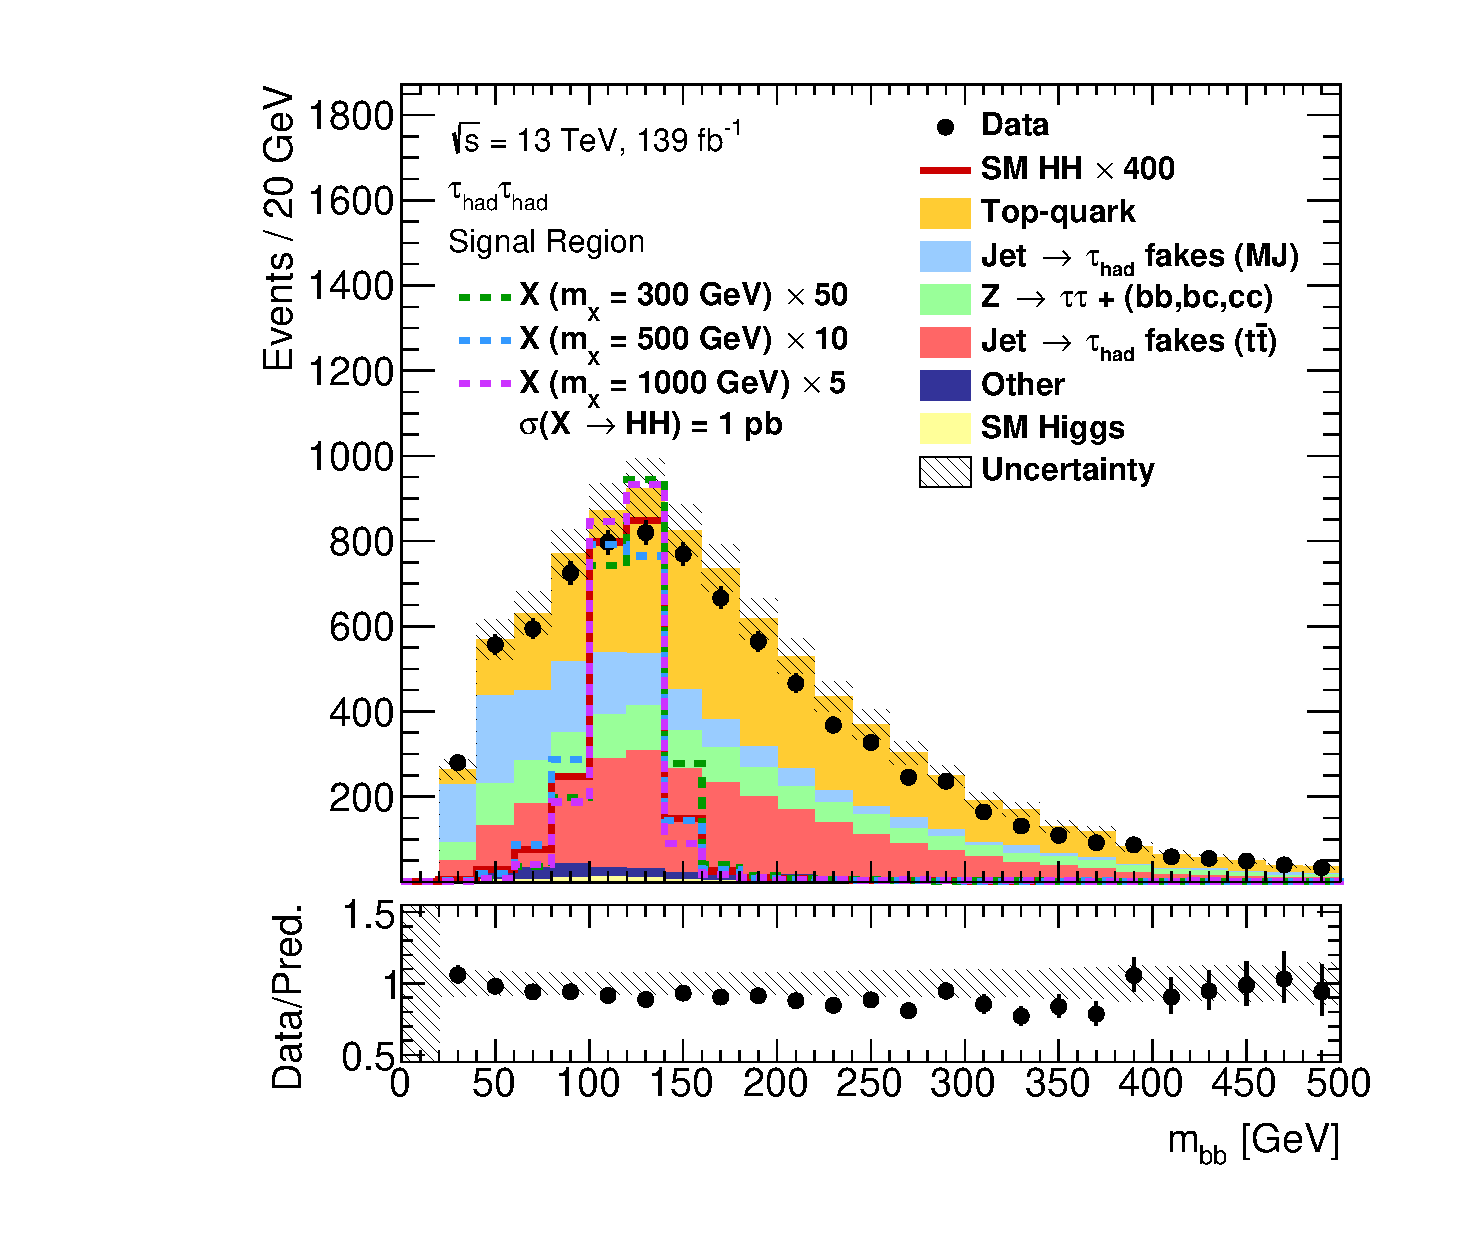
\includegraphics[width=\textwidth]{mva/prefit/Region_BMin0_incJet1_distmBB_J2_Y2015_DLLOS_T2_SpcTauHH_L0_Prefit}
  \end{subfigure}

  \begin{subfigure}[t]{.48\textwidth}
    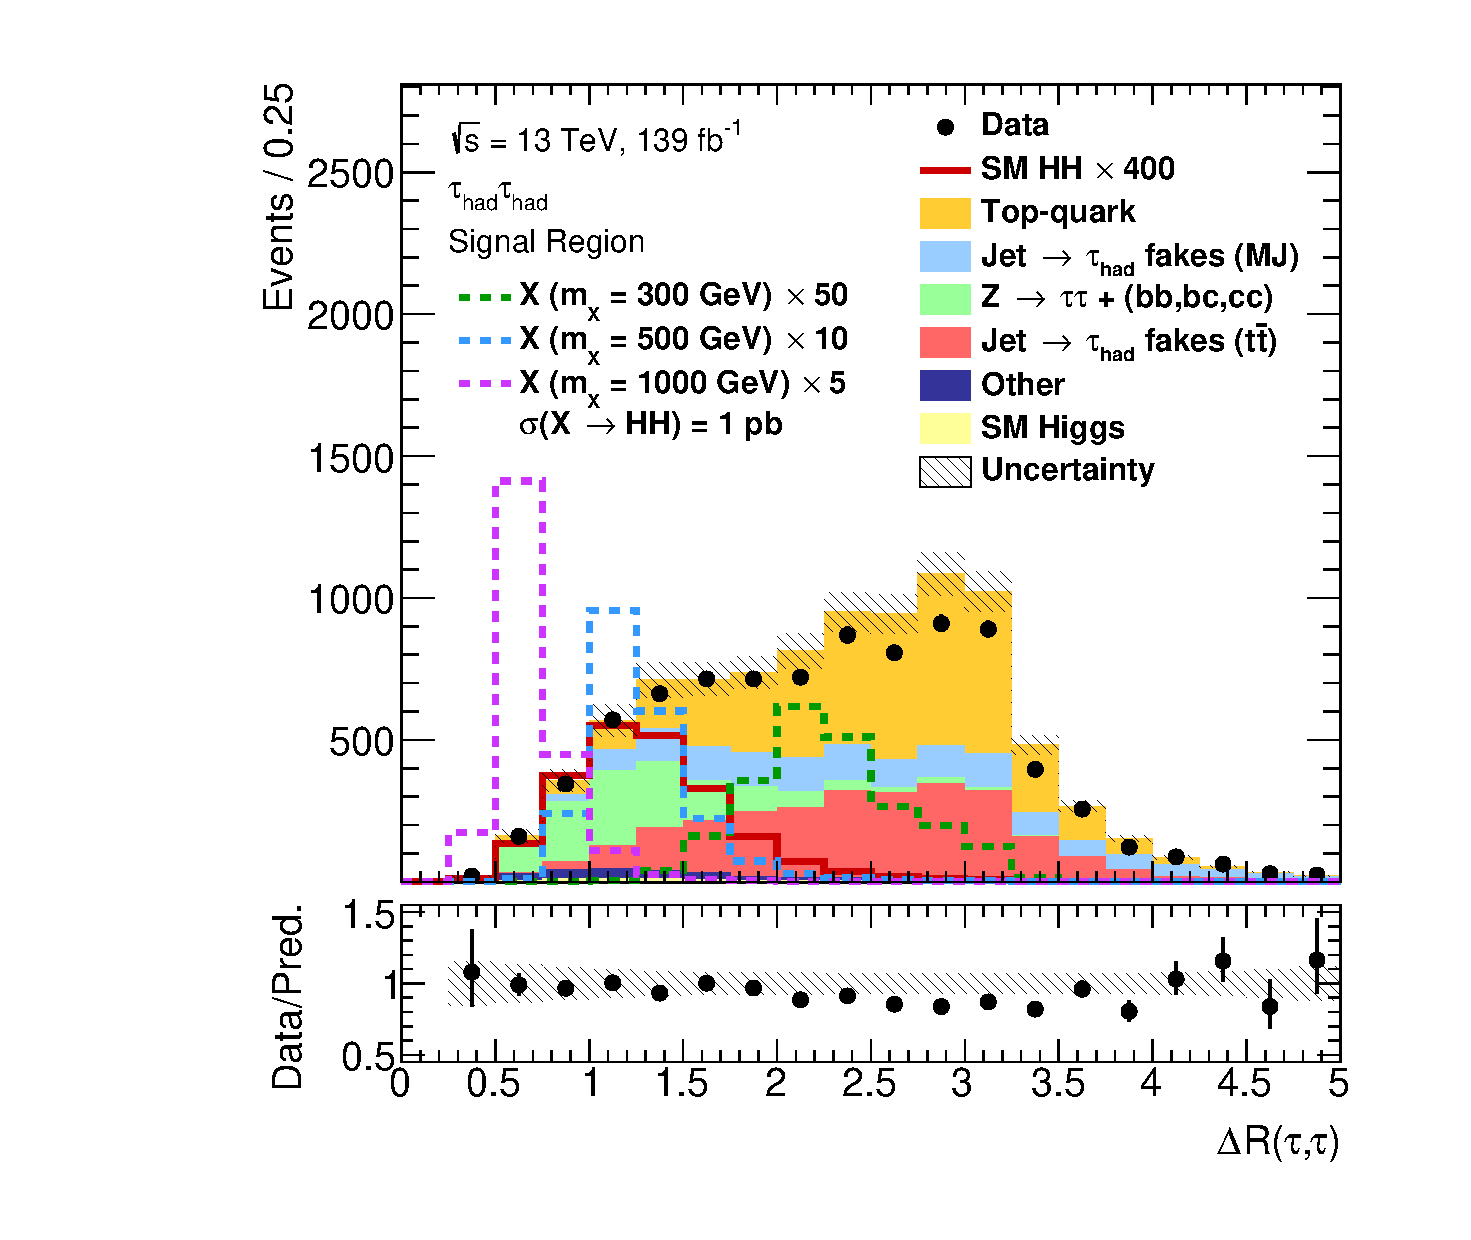
\includegraphics[width=\textwidth]{mva/prefit/Region_BMin0_incJet1_distdRTauTau_J2_Y2015_DLLOS_T2_SpcTauHH_L0_Prefit}
  \end{subfigure}\hfill %
  \begin{subfigure}[t]{.48\textwidth}
    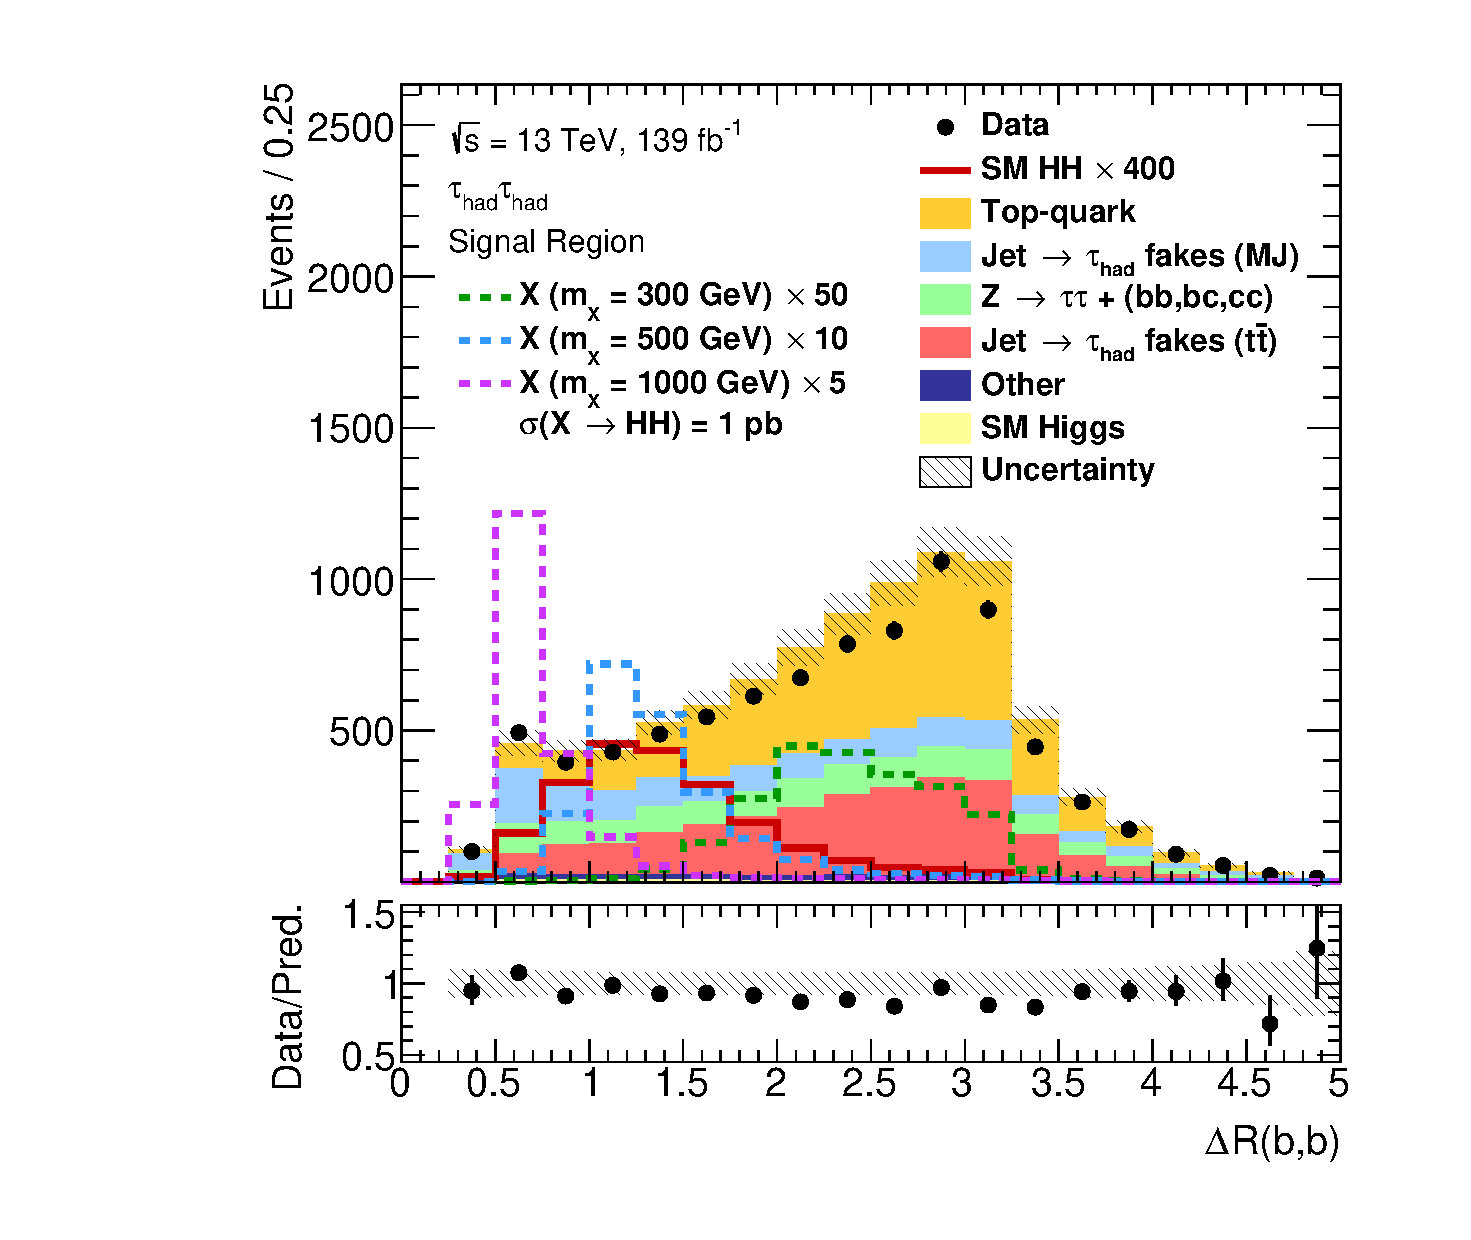
\includegraphics[width=\textwidth]{mva/prefit/Region_BMin0_incJet1_distdRBB_J2_Y2015_DLLOS_T2_SpcTauHH_L0_Prefit}
  \end{subfigure}

  \begin{subfigure}[t]{.48\textwidth}
    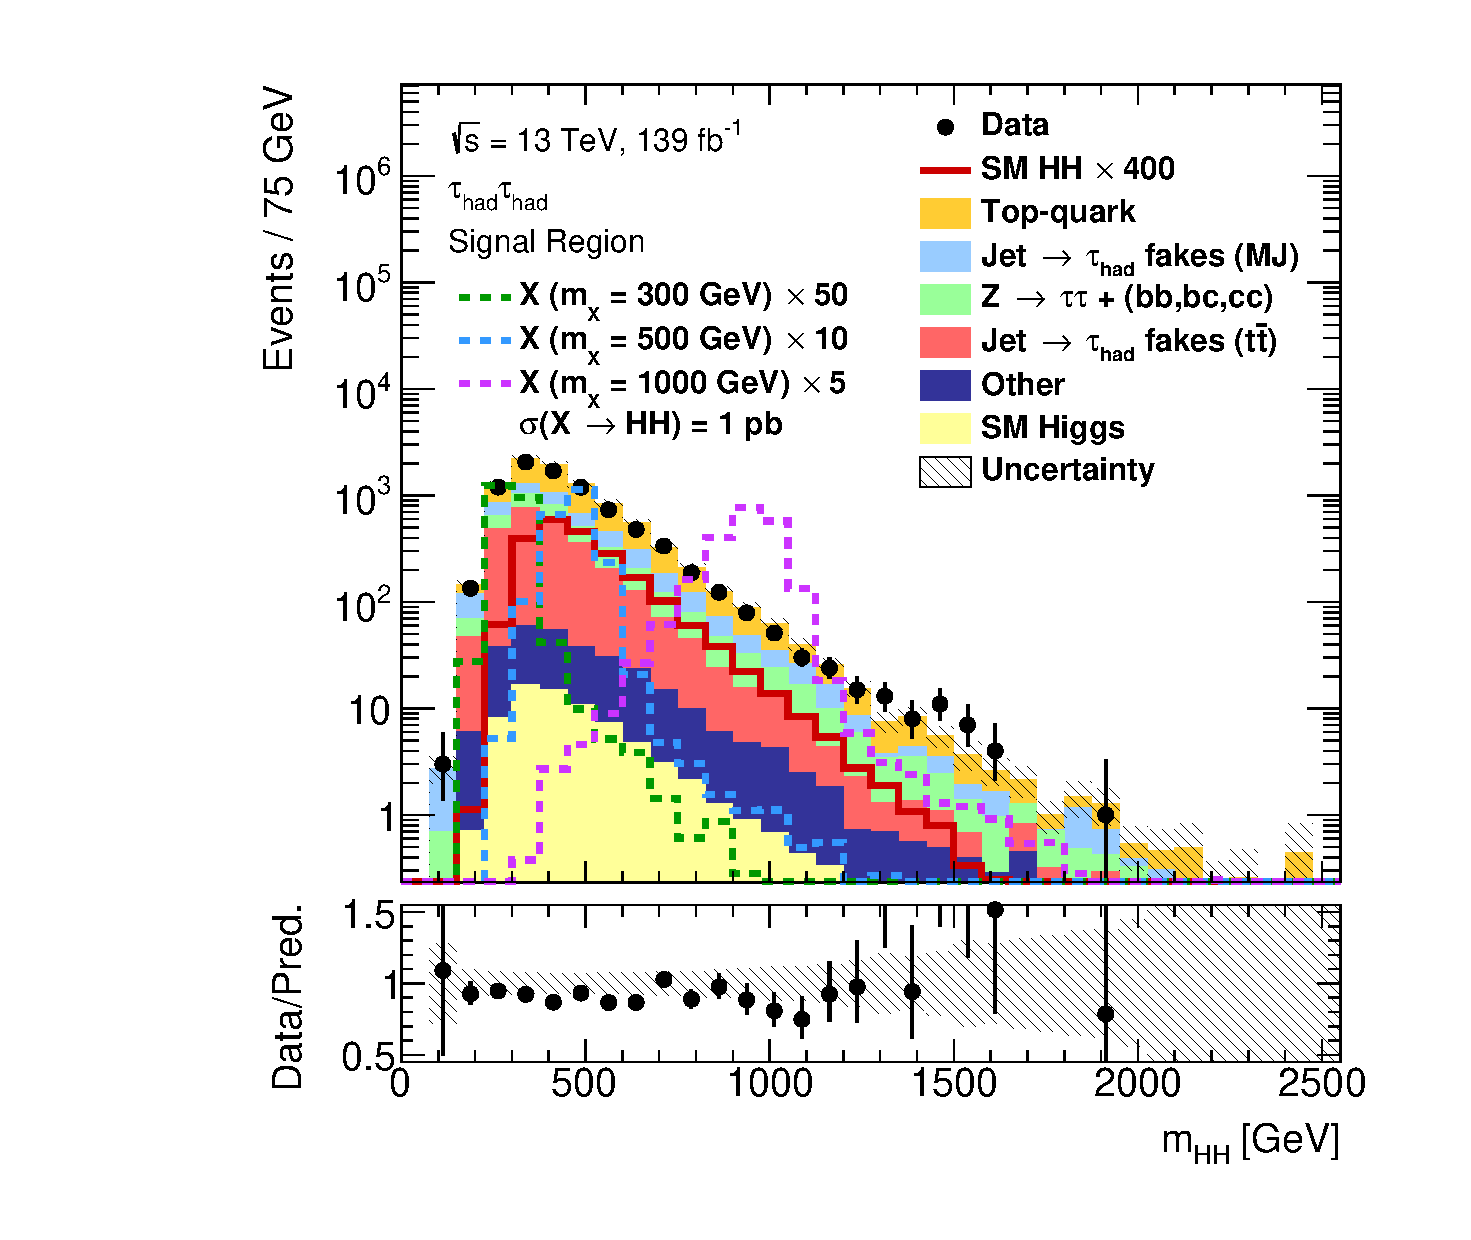
\includegraphics[width=\textwidth]{mva/prefit/Region_BMin0_incJet1_distmHH_J2_Y2015_DLLOS_T2_SpcTauHH_L0_Prefit_logy}
  \end{subfigure}

  \caption{Distributions of the MVA input variables in the SR of the
    \hadhad-channel prior to the maximum likelhood fit. The
    uncertainty bands include all statistical and systematic
    uncertainties of the background model. The resonant and
    non-resonant \HH signals are scaled by arbitrary factors for visibility.}
  \label{fig:mva_inputs}
\end{figure}


\subsection{Extraction of the non-resonant signal using Boosted
  Decision Trees in the \hadhad channel}
\label{sec:mva_smbdt}

The extraction of the non-resonant \HH signal is performed by training
BDTs to perform binary classification, distinguishing the signal
process, $\HH \to \bbtautau$, from the background. Events in the
2~$b$-tag preselection region of the \hadhad channel are used to train
the BDTs. The training uses simulation of the non-resonant \HH
production as the \emph{signal class}; the combination of all
backgrounds considered in the analysis as the \emph{background class}.
The individual background processes, which are estimated from
simulation or data (multi-jet), are weighted according to their
relative cross-sections. The implementation of the BDT algorithm in
the \emph{Toolkit for Multivariate Data Analysis}
(TMVA)~\cite{Hocker:2007ht} is used.

The BDT configuration is optimised using a random grid search. For
every hyperparameter of the algorithm a set of parameter values to
test is defined. All possible combinations of parameters values define
the parameter grid from which configurations are drawn randomly (with
replacement). The expected performance of the configuration is
evaluated using 5-fold cross validation separately on even- and
odd-numbered events.

The hyperparameter grid is defined
in~\Cref{tab:hyperparameter_grid_bdt}. The Gini index is used as the
splitting criterion in the decision tree algorithm, testing 400
possible cuts on input variables for every branching of the tree. The
total number of signal and background events are ensured to be equal
by rescaling of the event weights prior to the training. Other
settings remain at the default values of TMVA~v4.2.1~(ROOT~6.16/00).

\begin{table}[htbp]
  \centering
  \begin{tabular}{ll}
  \toprule
  Hyperparameter & Values considered \\
  \midrule
  Number of trees & 200, 400, 800, 1000, \underline{1500}, 2000 \\[0.1em]
  Tree depth & 1, \underline{2}, 3 \\[0.1em]
  Minimum node size & \SI{0.01}{\percent}, \SI{0.1}{\percent}, \underline{\SI{1}{\percent}}, \SI{5}{\percent} \\[0.1em]
  Boosting algorithm & \underline{Gradient Boosting}, AdaBoost \\[0.1em]
  Learning rate & 0.01, 0.02, 0.04, 0.08, 0.1, 0.15, \underline{0.2}, 0.3, 0.4 \\[0.1em]
  Ignore negatively weighted events & \underline{Yes}, No \\
  \bottomrule
\end{tabular}

%%% Local Variables:
%%% mode: latex
%%% TeX-master: "../phd_thesis"
%%% End:

  \caption{Hyperparameter grid used in the random grid search. The
    underlined values show the final configuration after
    optimisation.}
  \label{tab:hyperparameter_grid_bdt}
\end{table}

The metric used for optimisation is the area under the \emph{receiver
  operating characteristic} curve (ROC-AUC). The ROC curve is
defined\footnote{The ROC curve relates the true positive rate
  ($\varepsilon_\text{s}$) and false positive rate
  ($\varepsilon_\text{b}$) given varying thresholds on the output of a
  binary classifier. The definition used here uses conventions
  commonly used in HEP to express this relationship.} as the
parametric curve given by
$(x, y) = \left( \varepsilon_{\text{s}}(t), 1 -
  \varepsilon_{\text{b}}(t) \right)$, where $t$ is a lower threshold
applied on the score of a classifier, and $\varepsilon_\text{s}$ /
$\varepsilon_\text{b}$ the signal and background efficiency of this
selection, respectively. A value of the ROC-AUC of 1 indicates perfect
classification, while a value of 0.5 randomly assigned classes. The
ROC-AUC is chosen as the metric to be optimised as it summarises the
classifier's performance over all possible working points,
i.e.~choices of thresholds on the classifier output~\cite{james13}.

In total, approximately 1600 unique BDT configurations are tested
during the model selection process. The steps described in the
following are applied on the datasets containing even- and
odd-numbered events separately. The 5-fold CV approach described
in~\Cref{sec:mva_crossvalidation} is used to evaluate the performance
of a given hyperparameter configuration. For a fixed configuration the
ROC-AUC average and standard deviation is calculated over all
iterations of the CV.

Out of all evaluated configurations, the ROC-AUC of the 200 best
performing model configurations are statistically indistinguishable
based on the CV results. In the absence of a clearly preferred
configuration, the highest ranking configuration with the smallest
maximum tree depth is chosen. A smaller tree depth, effectively
limiting the number variable interactions used in the
classifier~\cite{hastie09}, is chosen to be less reliant on the
quality of the modelling of higher order variable interactions in the
training data.

The chosen configuration, shown in~\Cref{tab:hyperparameter_grid_bdt},
is 5th and 7th ranking with a ROC-AUC of \num{0.9803 +- 0.0008} and
\num{0.9787 +- 0.0012} in CV on even- and odd-numbered events,
respectively. In both cases the same configuration is the highest
ranking one with a tree depth of 2. After choosing the configuration,
the classifiers are re-trained on the entirety of their respective
outer folds, providing the final classifiers to extract the SM \HH
signal.

It should be noted that the model selection should be done
independently on both outer folds of the CV, typically leading to two
different configuration choices for even- and odd-numbered events, to
be free of model selection bias. The decision rule was not fixed a
priori, thus it cannot be excluded that the results informed the final
decision. This effect, however, is assumed to be negligible given the
large overlap of the best ranking configurations.\todo{Write properly}

\todo[inline]{Performance? ROC and distribution of SMBDT.}


\begin{table}[htbp]
  \centering

  \caption{Variable importance BDT}
  \label{tab:variable_importance_bdt}
\end{table}





\subsection{Extraction of resonant signals with parametric neural networks}
\label{sec:mva_pnn}


Note that 375 was excluded from the training


\begin{figure}[htbp]
  \centering

  \begin{subfigure}[t]{.49\textwidth}
    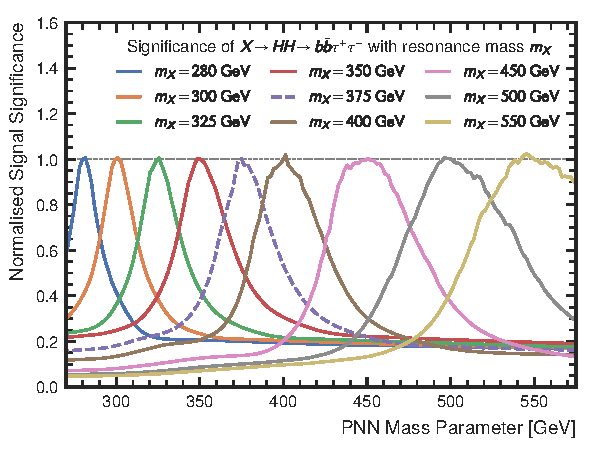
\includegraphics[width=\textwidth]{mva/detuning}
    \caption{Response of final PNN configuration used in the search
      for resonant production of \HH.}
  \end{subfigure}\hfill%
  \begin{subfigure}[t]{.49\textwidth}
    \centering
    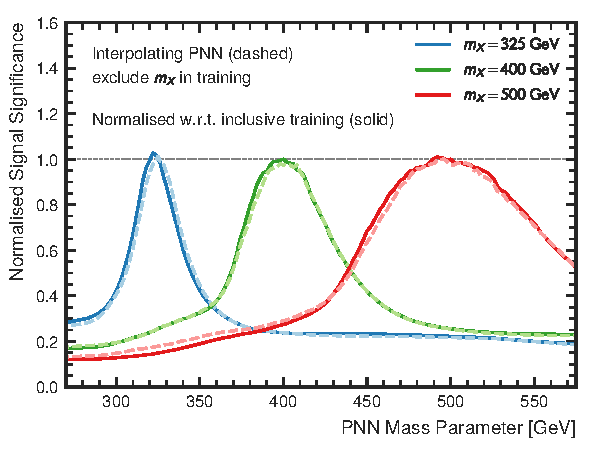
\includegraphics[width=\textwidth]{mva/interpolation}
    \caption{Comparison of PNN before hyperparameter optimisation when
      including (solid) and excluding (dashed) certain resonance
      masses in training.}
  \end{subfigure}

  \caption{Expected signal significance of a scalar resonance with
    mass \mX as a function of the PNN mass parameter. The significance
    is estimated by binning the PNN score for a given value of the
    parameter and adding the Asimov significance of all bins in
    quadrature. Only statistical uncertainties are considered. The
    binning is determined by an algorithm that will be described
    in~\Cref{sec:binning_alg}. The curves are scaled such that the
    significance is 1 when the PNN mass parameter is equal to \mX of
    the hypothesis under test. Dashed lines correspond to signal mass
    hypotheses that were not included in the PNN training.}
  \label{fig:pnn_properties}
\end{figure}


\begin{table}[htbp]
  \centering
  \begin{tabular}{ll}
  \toprule
  Hyperparameter & Values considered \\
  \midrule
  Epochs & 50, 100, \underline{200}, 400 \\[0.1em]
  Batch size & 64, \underline{128}, 256 \\[0.1em]
  Learning rate & 0.01, 0.02, 0.05, 0.1, \underline{0.2} \\[0.1em]
  Learning rate decay & $10^{-6}$, \underline{$10^{-5}$}, $10^{-4}$, $10^{-3}$ \\[0.1em]
  Number of hidden layers & 1, 2, 3, \underline{4}, 5 \\[0.1em]
  Layer size (first hidden layer) & 16, 32, 64, \underline{128} \\[0.1em]
  Layer size (last hidden layer$^*$) & \underline{16}, 32, 64, 128 \\
  Layer size (other hidden layers$^\dagger$) & 16, 32, 64, \underline{128} \\[0.1em]
  \bottomrule
\end{tabular}

%%% Local Variables:
%%% mode: latex
%%% TeX-master: "../phd_thesis"
%%% End:

  \caption{Hyperparameter grid. $\dagger$: Only applicable if the
    number of hidden layers is larger than 1 and 2, respectively.}
  \todo[inline]{Explain the layer size business}
  \label{tab:hyperparameter_grid_pnn}
\end{table}


Signal spectra connected to one or more physics parameters.

Input parameter: resonance mass \mX

Input parameter + input variables are inputs to the NN

Standardised by subtracting median and dividing by interquartile range.

Keras~\cite{keras}, Tensorflow\cite{tensorflow2015-whitepaper},
lwtnn~\cite{lwtnn}.


The metric used for optimisation of the PNN is the ROC-AUC for
$\mX = \SI{325}{\GeV}$. At this point there is a large overlap of
signal and background. Moreover, compared to other search channels
\bbtautau is most competitive in an intermediate mass range of 300 to
600 GeV.

About top 400 indistinguishable.

ROC-AUC (325) on even: \num{0.9764 +- 0.0009} ROC-AUC (325) on odd:
\num{0.9754 +- 0.0009}




\todo[inline]{Optimisation}
\todo[inline]{Performance: Detuning studies}


\subsection{Others?}

\todo[inline]{Variable ranking}


%%% Local Variables:
%%% mode: latex
%%% TeX-master: "../../phd_thesis"
%%% End:
